\section{Event Structure Semantics of DyNetKAT}
In this section, first, we introduce Normal DyNetKAT grammar.
Then we define different constructions on labeled event structures
which will be used to provide denotational semantics for Normal
DyNetKAT terms.

\subsection{Normal DyNetKAT}
We define the Normal DyNetKAT grammar as follows:
\begin{align*}
    F ::= & \alpha\cdot\pi                                                                           \\
    D ::= & \bot ~|~ F;D ~|~ x?F;D ~|~ x!F;D ~|~ D \parallel D ~|~ D \oplus D ~|~ \delta_{\mc{L}}(D) \\
          & \mc{L} = \s{c ~|~ c ::= x?F ~|~ x!F}
\end{align*}
Lemma 9 in \cite{dynetkat} says that for a given guarded DyNetKAT term
$p$ there exists a DyNetKAT term in normal form $q$ for which we have:
\begin{equation*}
    E_{DNK} \vdash p \equiv q
\end{equation*}
where $E_{DNK}$ is DyNetKAT axiom system.

\subsection{Constructions on Labeled Event Structures \cite{es}}
We use $(\e,\e)$ to denote an empty labeled event structure with
an empty set of events and an empty set of labels.
In the following, we define four types of constructions on labeled 
event structures.

\subsubsection{Prefix}

\begin{definition}
    Let $(\mr{E},L,l)$ be a labelled event structure.
    Let $\alpha$ be a label.
    Define $\alpha(\mr{E},L,l)$ to be a labelled event structure 
    $(\alpha \mr{E},L',l')$
    with labels:
    \begin{align*}
        L' = \s{\alpha} \cup L
    \end{align*}
    and
    $$
        l'(e') = \begin{cases}
            \alpha & \text{if } e' = (0,\alpha) \\
            l(e)   & \text{if } e' = (1,e)
        \end{cases}
    $$
    for all $e' \in E'$.
\end{definition}

\subsubsection{Sum}

\begin{definition}
    Let $\mr{E_0} = (E_0,\#_0,\vdash_0,L_0,l_0)$ and
    $\mr{E_1} = (E_1,\#_1,\vdash_1,L_1,l_1)$ be labelled event structures.
    Their sum $\mr{E_0} + \mr{E_1}$, is defined to be the structure $(E,\#,\vdash,l)$
    with events $E = \s{(0,e)|e \in E_0} \cup \s{(1,e)|e \in E_1}$,
    the disjoint union of sets $E_0$ and $E_1$,
    with injections $\iota_k: E_k \rightarrow E$, given by
    $\iota_k(e) = (k,e)$, for $k=0,1$, conflict relation
    \begin{align*}
        e \# e' \iff & \exists e_0,e_0'. e = \iota_0(e_0)
        \wedge e' = \iota_0(e_0') \wedge e_0 \#_0e_0'                       \\
                     & \text{or } \exists e_1,e_1'. e = \iota_1(e_1) \wedge
        e' = \iota_1(e_1') \wedge e_1 \#_1 e_1'                             \\
                     & \text{or } \exists e_0,e_1.(e=\iota_1(e_0)
        \wedge e' =\iota_1(e_1)) \text{ or }
        (e'=\iota_1(e_0) \wedge e =\iota_1(e_1))
    \end{align*}
    and enabling relation
    \begin{align*}
        X \vdash e \iff & X \in Con \wedge e \in E \wedge                   & \\
                        & (\exists X_0 \in Con_0,e_0 \in E_0.X = \iota_0X_0
        \wedge e = \iota_0(e_0) \wedge X_0 \vdash_0 e_0) \text{ or }          \\
                        & (\exists X_1 \in Con_1,e_1 \in E_1.X = \iota_1X_1
        \wedge e = \iota_1(e_1) \wedge X_1 \vdash_1 e_1)                      \\
    \end{align*}
    We define the set of labels as $L_0 \cup L_1$ and the labelling function as:
    $$
        l(e) = \begin{cases}
            l_0(e_0) & \text{ if } e = \iota_0(e_0) \\
            l_1(e_1) & \text{ if } e = \iota_1(e_1)
        \end{cases}
    $$
\end{definition}

\subsubsection{Product}
In the product of two event structures, their events of synchronization are those pairs of events $(e_0,e_1)$, one from each event structure;
if $e_0$ is labelled $\alpha_0$ and $e_1$ is labelled $\alpha_1$ the synchronization event is
then labelled $(\alpha_0,\alpha_1)$.
Events need not synchronize however; an event in one component may not synchronize with
any event in the other.
We shall use events of the form $(e_0,*)$ to stand for the occurrence of an event $e_0$
from one component unsynchronized with any event of the other.
Such an event will be labeled by $(\alpha_0,*)$ where $\alpha_0$ is the original label of $e_0$
and * is a sort of undefined.

\begin{definition}
    Let $\mr{E_0} = (E_0,\#_0,\vdash_0,L_0,l_0)$ and
    $\mr{E_1} = (E_1,\#_1,\vdash_1,L_1,l_1)$
    be labeled event structures.
    Define their product $\mr{E_0} \times \mr{E_1}$ to be the structure $\mr{E} = (E,\#,\vdash,L,l)$
    consisting of events $E$ of the form
    \begin{align*}
        E_0 \times_* E_1 =
        \s{(e_0,*)|e_0 \in E_0}
        \cup \s{(*,e_1)|e_1 \in E_1}
        \cup \s{(e_0,e_1)| e_0 \in E_0 \wedge e_1 \in E_1}
    \end{align*}
    with projections $\pi_i : E \rightarrow_* E_i$,
    given by $\pi_i(e_0,e_1) = e_i$, for $i=0,1$, reflexive conflict relation $\doublevee$ given by
    \begin{align*}
        e \doublevee e' \iff \pi_0(e) \doublevee_0 \pi_0(e') \text{ or }
        \pi_1(e) \doublevee_1 \pi_1(e')
    \end{align*}
    for all $e,e'$ we use $Con$ for the conflict-free finite sets,
    enabling relation $\vdash$ given by
    \begin{align*}
         & X \vdash e \iff X \in Con \wedge e \in E \wedge                  \\
         & (\pi_0(e)\text{ is defined } \Rightarrow \pi_0X\vdash_0\pi_0(e))
        \wedge (\pi_1(e)\text{ is defined } \Rightarrow \pi_1X\vdash_1\pi_1(e))
    \end{align*}
    Its set of labels is
    \begin{align*}
        L_0 \times_* L_1 = \s{ (\alpha_0,*)|\alpha_0 \in L_0}
        \cup \s{(*,\alpha_1)|\alpha_1 \in L_1}
        \cup \s{(\alpha_0,\alpha_1)|\alpha_0 \in L_0 \wedge \alpha_1 \in L_1}
    \end{align*}
    with projections: $\lambda_i: E \rightarrow_* E_i$ given by
    $\lambda_i(\alpha_0,\alpha_1) = \alpha_i$, for $i=0,1$.
    Its labeling function is defined to act on an event $e$ so
    \begin{align*}
        l(e) = (l_0\pi_0(e),l_1\pi_1(e))
    \end{align*}
\end{definition}

\subsubsection{Restriction}

\begin{definition}

    Let $\mr{E} = (E,\#,\vdash,L,l)$ be a labelled event structure.
    Let $\Lambda$ be a subset of labels.
    Define the restriction $\mr{E}\lceil \Lambda$ to be $(E',\#',\vdash',L\cap \Lambda,l')$
    where $(E',\#',\vdash')$ is the restriction of $(E,\#,\vdash)$
    to events $\s{e \in E|l(e) \in \Lambda}$ and the labeling function $l'$
    is the restriction of the original labeling function to the domain $L \cap \Lambda$.
\end{definition}

\subsection{Denotational Semantics of Normal DyNetKAT}

\begin{definition}
    Let $\mc{A}$ be an alphabet of letters of the form
    $\alpha \cdot \pi$,
    $x?F$, and $x!F$.
    We define the semantic map of Normal DyNetKAT terms
    $\sem{ \ }: D \ra \mathbb{E}$ where
    $\mathbb{E}$ is the set of all event structures with
    labels in $\mc{A}$ as follows:
    \begin{align*}
        \sem{\bot}      & = (\emptyset,\emptyset)                  \\
        \sem{\alpha; t} & = \alpha\sem{t}                        \\
        \sem{t_1 \oplus t_2}
                        & = \sem{t_1} + \sem{t_2}                  \\
        \sem{\delta_{\mc{L}}(t)}
                        & = \sem{t} \lceil (\mc{A} \setminus \mc{L}) \\
        \sem{t_1 \parallel t_2}
                        & = \sem{t_1} \times \sem{t_2}
    \end{align*}
    Where $\mc{L}$ is a subset of $\mc{A}$.
\end{definition}

\subsection{Examples}
In the following, we provide some examples to illustrate
how the prefix, sum, and product operators can be used to 
compose event structures.
For simplicity, here we use $a,b,c$ to denote DyNetKAT actions.

\begin{example}
    Let $a,b\in \mc{A}$ be some DyNetKAT actions and $a;b$ a
    normal DyNetKAT term.
    $\mr{E} = \sem{a;b}$ is an event structure
    $(E,\#,\vdash,L,l)$ where:
    \begin{align*}
        E  & = \s{(0,a),(1,0,b)}                       \\
        \# & = \emptyset                               \\
           & \e \vdash (0,a), \s{(0,a)} \vdash (1,0,b) \\
        L  & = \s{a,b}                                 \\
           & l((0,a)) = a, l((1,0,b)) = b              
    \end{align*}
    The following diagram shows configurations of $\mr{E}$:
    \begin{center}
        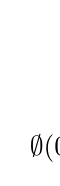
\begin{tikzpicture}[scale=0.8]
            \crd[right]{0}{0}{$\emptyset$}
            \crd[right]{0}{1}{$\s{(0,a)}$}
            \crd[right]{0}{2}{$\s{(0,a),(1,0,b)}$}
            \draw [ultra thick] (0,0) -- (0,1);
            \draw [ultra thick] (0,1) -- (0,2);
        \end{tikzpicture}
    \end{center}
\end{example}

\begin{example}
    Let $a,b\in \mc{A}$ be some DyNetKAT actions and $a\oplus b$ a
    normal DyNetKAT term.
    $\mr{E} = \sem{a\oplus b}$ is an event structure
    $(E,\#,\vdash,L,l)$ where:
    \begin{align*}
        E & = \s{(0,a),(1,b)}                \\
          & (0,a) \# (1,b) , (1,b) \# (0,a)  \\
          & \e \vdash (0,a), \e \vdash (1,b) \\
        L & = \s{a,b}                        \\
          & l((0,a)) = a, l((1,b)) = b       
    \end{align*}
    The following diagram shows configurations of $\mr{E}$:
    \begin{center}
        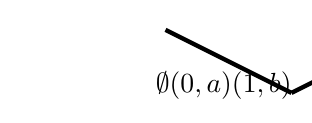
\begin{tikzpicture}[scale=0.8]
            \crd[above]{0}{0}{$\emptyset$}
            \crd[above]{-2}{1}{$\s{(0,a)}$}
            \crd[above]{2}{1}{$\s{(1,b)}$}
            \draw [ultra thick] (0,0) -- (-2,1);
            \draw [ultra thick] (0,0) -- (2,1);
        \end{tikzpicture}
    \end{center}
\end{example}


\begin{example}
    Let $a,b\in \mc{A}$ be some DyNetKAT actions and $a\parallel b$ a
    normal DyNetKAT term.
    $\mr{E} = \sem{a\parallel b}$ is an event structure
    $(E,\#,\vdash,L,l)$ where:
    \begin{align*}
        E  & = \s{(a,*),(*,b),(a,b)}                           \\
        \# & = \e                                              \\
           & \e \vdash (a,*), \e \vdash (*,b),\e \vdash (a,b)  \\
        L  & = \s{(a,*),(*,b),(a,b)}                           \\
           & l((a,*)) = (a,*), l((*,b)) = (*,b),l((a,b))=(a,b) 
    \end{align*}
    The following diagram shows configurations of $\mr{E}$:
    \begin{center}
        \begin{tikzpicture}[scale=0.8]
            \crd[above]{0}{0}{$\emptyset$}
            \crd[left]{-2}{1}{$\s{(a,*)}$}
            \crd[right]{2}{1}{$\s{(*,b)}$}
            \crd[above]{0}{2}{$\s{(a,*),(*,b)}$}
            \crd[above]{2}{3}{$\s{(a,b)}$}
            \draw [ultra thick] (0,0) -- (-2,1);
            \draw [ultra thick] (0,0) -- (2,1);
            \draw [ultra thick] (2,1) -- (0,2);
            \draw [ultra thick] (-2,1) -- (0,2);
            \draw [ultra thick] (0,0) -- (2,3);
        \end{tikzpicture}
    \end{center}
\end{example}